\documentclass[]{article}
\usepackage{lmodern}
\usepackage{amssymb,amsmath}
\usepackage{ifxetex,ifluatex}
\usepackage{fixltx2e} % provides \textsubscript
\ifnum 0\ifxetex 1\fi\ifluatex 1\fi=0 % if pdftex
  \usepackage[T1]{fontenc}
  \usepackage[utf8]{inputenc}
\else % if luatex or xelatex
  \ifxetex
    \usepackage{mathspec}
    \usepackage{xltxtra,xunicode}
  \else
    \usepackage{fontspec}
  \fi
  \defaultfontfeatures{Mapping=tex-text,Scale=MatchLowercase}
  \newcommand{\euro}{€}
\fi
% use upquote if available, for straight quotes in verbatim environments
\IfFileExists{upquote.sty}{\usepackage{upquote}}{}
% use microtype if available
\IfFileExists{microtype.sty}{%
\usepackage{microtype}
\UseMicrotypeSet[protrusion]{basicmath} % disable protrusion for tt fonts
}{}
\usepackage[margin=.5in]{geometry}
\usepackage{color}
\usepackage{fancyvrb}
\newcommand{\VerbBar}{|}
\newcommand{\VERB}{\Verb[commandchars=\\\{\}]}
\DefineVerbatimEnvironment{Highlighting}{Verbatim}{commandchars=\\\{\}}
% Add ',fontsize=\small' for more characters per line
\usepackage{framed}
\definecolor{shadecolor}{RGB}{248,248,248}
\newenvironment{Shaded}{\begin{snugshade}}{\end{snugshade}}
\newcommand{\KeywordTok}[1]{\textcolor[rgb]{0.13,0.29,0.53}{\textbf{{#1}}}}
\newcommand{\DataTypeTok}[1]{\textcolor[rgb]{0.13,0.29,0.53}{{#1}}}
\newcommand{\DecValTok}[1]{\textcolor[rgb]{0.00,0.00,0.81}{{#1}}}
\newcommand{\BaseNTok}[1]{\textcolor[rgb]{0.00,0.00,0.81}{{#1}}}
\newcommand{\FloatTok}[1]{\textcolor[rgb]{0.00,0.00,0.81}{{#1}}}
\newcommand{\CharTok}[1]{\textcolor[rgb]{0.31,0.60,0.02}{{#1}}}
\newcommand{\StringTok}[1]{\textcolor[rgb]{0.31,0.60,0.02}{{#1}}}
\newcommand{\CommentTok}[1]{\textcolor[rgb]{0.56,0.35,0.01}{\textit{{#1}}}}
\newcommand{\OtherTok}[1]{\textcolor[rgb]{0.56,0.35,0.01}{{#1}}}
\newcommand{\AlertTok}[1]{\textcolor[rgb]{0.94,0.16,0.16}{{#1}}}
\newcommand{\FunctionTok}[1]{\textcolor[rgb]{0.00,0.00,0.00}{{#1}}}
\newcommand{\RegionMarkerTok}[1]{{#1}}
\newcommand{\ErrorTok}[1]{\textbf{{#1}}}
\newcommand{\NormalTok}[1]{{#1}}
\usepackage{graphicx}
\makeatletter
\def\maxwidth{\ifdim\Gin@nat@width>\linewidth\linewidth\else\Gin@nat@width\fi}
\def\maxheight{\ifdim\Gin@nat@height>\textheight\textheight\else\Gin@nat@height\fi}
\makeatother
% Scale images if necessary, so that they will not overflow the page
% margins by default, and it is still possible to overwrite the defaults
% using explicit options in \includegraphics[width, height, ...]{}
\setkeys{Gin}{width=\maxwidth,height=\maxheight,keepaspectratio}
\ifxetex
  \usepackage[setpagesize=false, % page size defined by xetex
              unicode=false, % unicode breaks when used with xetex
              xetex]{hyperref}
\else
  \usepackage[unicode=true]{hyperref}
\fi
\hypersetup{breaklinks=true,
            bookmarks=true,
            pdfauthor={Evan Oman},
            pdftitle={Statistical Inference Course Project Part 2},
            colorlinks=true,
            citecolor=blue,
            urlcolor=blue,
            linkcolor=magenta,
            pdfborder={0 0 0}}
\urlstyle{same}  % don't use monospace font for urls
\setlength{\parindent}{0pt}
\setlength{\parskip}{6pt plus 2pt minus 1pt}
\setlength{\emergencystretch}{3em}  % prevent overfull lines
\setcounter{secnumdepth}{0}

%%% Use protect on footnotes to avoid problems with footnotes in titles
\let\rmarkdownfootnote\footnote%
\def\footnote{\protect\rmarkdownfootnote}

%%% Change title format to be more compact
\usepackage{titling}
\setlength{\droptitle}{-2em}
  \title{Statistical Inference Course Project Part 2}
  \pretitle{\vspace{\droptitle}\centering\huge}
  \posttitle{\par}
  \author{Evan Oman}
  \preauthor{\centering\large\emph}
  \postauthor{\par}
  \predate{\centering\large\emph}
  \postdate{\par}
  \date{02/22/2015}




\begin{document}

\maketitle


\section{Introduction}

The ToothGrowth dataset provided by \(R\) is a dataset collected in
order to measure the effect on Guinea Pig tooth growth based on two
different delivery supplements at three different dosages. The dataset
consists of 60 observations with inputs: delivery methods(orange juice
or ascorbic acid) and dosage: .5, 1, or 2 mg; and output variable: tooth
length(more specifically the length of certain cells within the tooth).
We are asked to determine whether or not tooth growth is affected by
delivery method(supp) or by dosage(dose).

\section{Exploratory Analysis}

We begin by trying to get a rough idea of what the data looks like.
First we plot the tooth length by supp:

\begin{Shaded}
\begin{Highlighting}[]
\KeywordTok{library}\NormalTok{(ggplot2)}
\KeywordTok{data}\NormalTok{(ToothGrowth)}
\NormalTok{ToothGrowth$supp <-}\StringTok{ }\KeywordTok{as.factor}\NormalTok{(ToothGrowth$supp)}
\KeywordTok{ggplot}\NormalTok{(ToothGrowth, }\KeywordTok{aes}\NormalTok{(}\DataTypeTok{x=}\NormalTok{len)) +}
\StringTok{    }\KeywordTok{geom_histogram}\NormalTok{(}\DataTypeTok{fill =} \StringTok{"royalblue"}\NormalTok{, }\DataTypeTok{binwidth =} \FloatTok{0.75}\NormalTok{) +}
\StringTok{    }\KeywordTok{facet_wrap}\NormalTok{( ~}\StringTok{ }\NormalTok{supp, }\DataTypeTok{ncol=}\DecValTok{1}\NormalTok{)}
\end{Highlighting}
\end{Shaded}

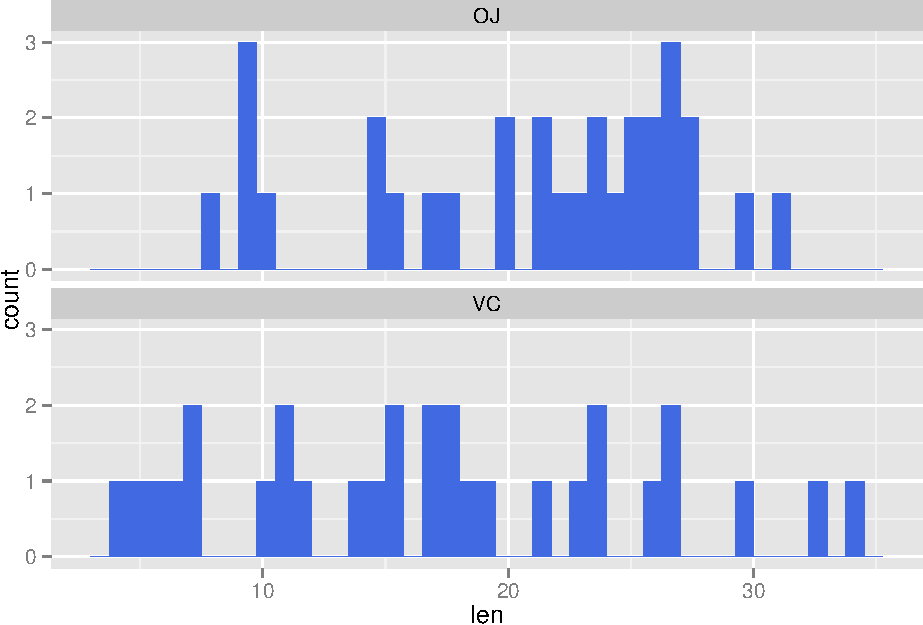
\includegraphics{SI-Proj2_files/figure-latex/unnamed-chunk-1-1.pdf}

Based on this plot I would say that there is definitely a difference in
the variance of the tooth length between VC or OJ, but I am not exactly
sure if there is a statistically significant difference between the
means. Now we plot tooth length by dosage:

\begin{Shaded}
\begin{Highlighting}[]
\NormalTok{ToothGrowth$dose <-}\StringTok{ }\KeywordTok{as.factor}\NormalTok{(ToothGrowth$dose)}
\KeywordTok{ggplot}\NormalTok{(ToothGrowth, }\KeywordTok{aes}\NormalTok{(}\DataTypeTok{x=}\NormalTok{len)) +}
\StringTok{    }\KeywordTok{geom_histogram}\NormalTok{(}\DataTypeTok{fill =} \StringTok{"royalblue"}\NormalTok{, }\DataTypeTok{binwidth =} \FloatTok{0.75}\NormalTok{) +}
\StringTok{    }\KeywordTok{facet_wrap}\NormalTok{( ~}\StringTok{ }\NormalTok{dose, }\DataTypeTok{ncol=}\DecValTok{1}\NormalTok{)}
\end{Highlighting}
\end{Shaded}

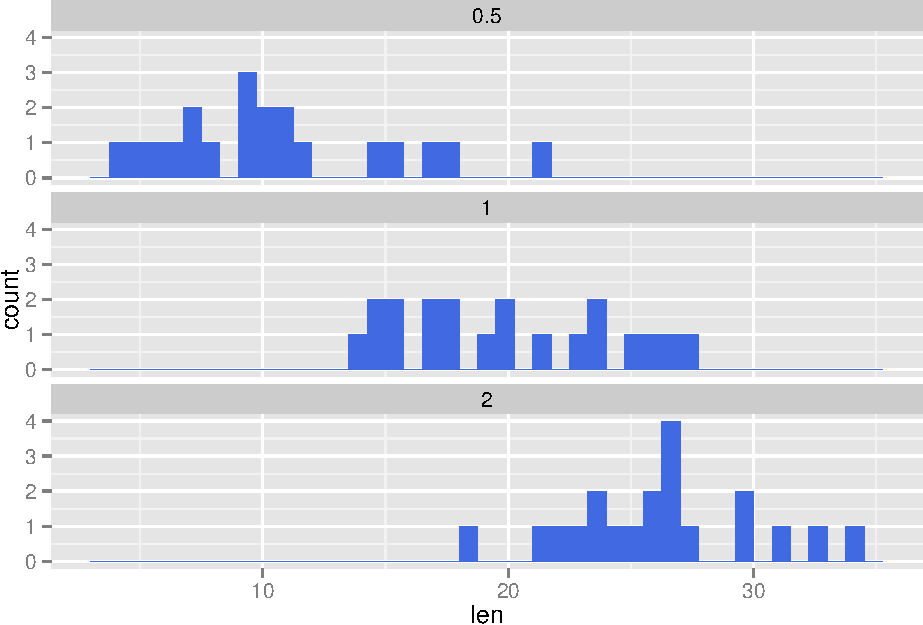
\includegraphics{SI-Proj2_files/figure-latex/unnamed-chunk-2-1.pdf}

Here it is pretty clear that there is a noticable difference between the
means of each dosage.

\section{Hypothesis Testing}

We will now perform hypothesis testing to answer concretely the
questions posed above. For these tests we will use a T
distribution(since we have a very small sample size) and an \(\alpha\)
level of .05.

First we will look at the supp variable. We define the hypotheses to be:

\begin{itemize}
\item $H_0$ : The means $\mu_{VC}$ and $\mu_{OJ}$ are the same, such that $\mu_{VC} - \mu_{OJ} = 0$
\item $H_a$ : The means $\mu_{VC}$ and $\mu_{OJ}$ are not the same, such that $\mu_{VC} - \mu_{OJ} \neq 0$
\end{itemize}

Here we can simply use a two-tailed T test with \(R\):

\begin{Shaded}
\begin{Highlighting}[]
\KeywordTok{t.test}\NormalTok{(len ~}\StringTok{ }\NormalTok{supp, }\DataTypeTok{data =} \NormalTok{ToothGrowth)$p.value}
\end{Highlighting}
\end{Shaded}

\begin{verbatim}
## [1] 0.06063451
\end{verbatim}

Thus we can see that our \(p\) value is .0606. Then since
\(p > \alpha\), we fail to reject the null hypothesis that the means are
the same(though we do so just barely). Thus we can conclude that, in our
sample, the supp variable does not affect the length of Guinea Pig teeth
in a statistically significant manner.

Next we will consider the dosages given by the dose variable. Since this
measurement is split into 3 levels, we will need to look at the
difference in means for .05 mg vs 1 mg, 1 mg vs 2 mg, and .5 mg vs 2
mg(note that if we were not limited to the methods introduced in this
course, this problem would be a prime candidate for ANOVA). The
following code makes three data sets based on the comparisons mentioned
above:

\begin{Shaded}
\begin{Highlighting}[]
\NormalTok{TG12 <-}\StringTok{ }\NormalTok{ToothGrowth[ToothGrowth$dose ==}\StringTok{ }\NormalTok{.}\DecValTok{5} \NormalTok{|}\StringTok{ }\NormalTok{ToothGrowth$dose ==}\StringTok{ }\DecValTok{1}\NormalTok{,]}
\NormalTok{TG13 <-}\StringTok{ }\NormalTok{ToothGrowth[ToothGrowth$dose ==}\StringTok{ }\DecValTok{1} \NormalTok{|}\StringTok{ }\NormalTok{ToothGrowth$dose ==}\StringTok{ }\DecValTok{2}\NormalTok{,]}
\NormalTok{TG23 <-}\StringTok{ }\NormalTok{ToothGrowth[ToothGrowth$dose ==}\StringTok{ }\NormalTok{.}\DecValTok{5} \NormalTok{|}\StringTok{ }\NormalTok{ToothGrowth$dose ==}\StringTok{ }\DecValTok{2}\NormalTok{,]}
\end{Highlighting}
\end{Shaded}

Now that we have our data we define our hypotheses as:

\begin{itemize}
\item $H_0^{i,j}$ : The means $\mu_{i}$ and $\mu_{j}$ are the same, such that $\mu_{i} - \mu_{j} = 0$
\item $H_a^{i,j}$ : The means $\mu_{i}$ and $\mu_{i}$ are not the same, such that $\mu_{i} - \mu_{j} \neq 0$
\end{itemize}

Where \(i,j \in \{1,2,3\}, \ i < j\). We can then perform T tests as we
did before on each of these 3 data sets:

\begin{Shaded}
\begin{Highlighting}[]
\KeywordTok{t.test}\NormalTok{(len ~}\StringTok{ }\NormalTok{dose, }\DataTypeTok{data =} \NormalTok{TG12)$p.value}
\end{Highlighting}
\end{Shaded}

\begin{verbatim}
## [1] 1.268301e-07
\end{verbatim}

\begin{Shaded}
\begin{Highlighting}[]
\KeywordTok{t.test}\NormalTok{(len ~}\StringTok{ }\NormalTok{dose, }\DataTypeTok{data =} \NormalTok{TG13)$p.value}
\end{Highlighting}
\end{Shaded}

\begin{verbatim}
## [1] 1.90643e-05
\end{verbatim}

\begin{Shaded}
\begin{Highlighting}[]
\KeywordTok{t.test}\NormalTok{(len ~}\StringTok{ }\NormalTok{dose, }\DataTypeTok{data =} \NormalTok{TG23)$p.value}
\end{Highlighting}
\end{Shaded}

\begin{verbatim}
## [1] 4.397525e-14
\end{verbatim}

Checking each of the \(p\) values, we see that each is well below our
\(\alpha\) level of .05 so we reject all three of our null hypotheses
and conclude that, in our sample, the dosage level correlates to a
statistically significant change in the length of Ginea Pig teeth.

\end{document}
